\phantomsection
\section*{Chapitre 1 : Le Minist\`ere de la Justice}\addcontentsline{toc}{section}{Chapitre 1 : Le Minist\`ere de la Justice}

\bigskip

Tout projet d'optimisation budgétaire commence par comprendre l'institution dont on pilote les crédits. Ce chapitre retrace l'évolution du Ministère de la Justice depuis 1955, décrit ses missions, et présente son organisation. Une attention particulière est portée à la Direction du Budget~-- interlocuteur direct de cette étude.
%================================================================
\phantomsection
\subsection*{1.1 \quad Historique et missions}
\addcontentsline{toc}{subsection}{1.1 Historique et missions}
%================================================================

%----------------------------------------------------------------
\phantomsection
\subsubsection*{1.1.1 \quad \'Evolution institutionnelle}
\addcontentsline{toc}{subsubsection}{1.1.1 \'Evolution institutionnelle}
%----------------------------------------------------------------

Le minist\`ere de la Justice occupe une place singuli\`ere dans l'architecture institutionnelle marocaine. H\'eritier d'une tradition juridique plurielle (islamique, coutumi\`ere et civiliste), il a connu depuis sa cr\'eation en 1955 plusieurs mutations profondes refl\'etant l'\'evolution du cadre constitutionnel et des priorit\'es de l'\'Etat. La Constitution de 2011 constitue un tournant d\'ecisif~: en consacrant l'ind\'ependance du pouvoir judiciaire et en cr\'eant le Conseil Sup\'erieur du Pouvoir Judiciaire (CSPJ), elle a red\'efini le p\'erim\`etre d'intervention du minist\`ere, recentr\'e d\'esormais sur les missions administratives, financi\`eres et logistiques d'appui au syst\`eme judiciaire \citep{MEF2015}.

Cette \'evolution s'est accompagn\'ee d'une r\'eforme progressive du syst\`eme judiciaire, articul\'ee autour de la Charte de la R\'eforme du Syst\`eme Judiciaire adopt\'ee en 2013, dont les axes ont \'et\'e d\'eclin\'es en programmes et actions budg\'etaires conform\'ement \`a la Loi Organique relative \`a la Loi de Finances n\textsuperscript{o}~130-13.

%----------------------------------------------------------------
\phantomsection
\subsubsection*{1.1.2 \quad Missions et attributions}
\addcontentsline{toc}{subsubsection}{1.1.2 Missions et attributions}
%----------------------------------------------------------------

Les missions du minist\`ere, telles que d\'efinies par le D\'ecret n\textsuperscript{o}~2.22.400 du 18~octobre~2022 relatif aux attributions et \`a l'organisation du minist\`ere de la Justice, s'articulent autour de quatre domaines principaux~:

\begin{itemize}
    \item \textbf{La gestion administrative et financi\`ere des juridictions}~: le minist\`ere assure la gestion des ressources humaines, financi\`eres et logistiques des tribunaux de l'ensemble du territoire national. Il supervise l'organisation du travail administratif des greffes et assure la coordination entre les services judiciaires et les services d\'econcentr\'es.

    \item \textbf{La gestion du patrimoine et des infrastructures judiciaires}~: construction, r\'ehabilitation et \'equipement des palais de justice et des \'etablissements p\'enitentiaires. Cette mission mobilise une part significative des cr\'edits d'investissement du minist\`ere.

\item \textbf{La transformation numérique et la modernisation du service judiciaire}~: pilotage de la transition numérique des juridictions, déploiement de plateformes dématérialisées et intégration des technologies de l’information dans les procédures judiciaires et administratives.

\item \textbf{La gestion des ressources humaines du personnel judiciaire et administratif}~: recrutement, formation, avancement et gestion pr\'evisionnelle des effectifs du corps des magistrats, des greffiers, des administrateurs et du personnel p\'enitentiaire.
\end{itemize}

Dans le cadre de la mise en \oe{}uvre de la Charte Nationale pour la Réforme du Système Judiciaire, le ministère poursuit l’édification d’une administration judiciaire professionnelle fondée sur la déconcentration administrative et financière. Le Projet de performance du PLF~2026 structure cette réforme autour de trois axes~: la modernisation de la législation, la facilitation de l’accès à la justice et la qualification de l’administration judiciaire \citep{MJNumerique2026}. Sur le plan numérique, la vision stratégique 2025--2030 vise à placer le justiciable au c\oe{}ur de la transformation en déployant une justice numérique efficace et transparente et en mobilisant l’intelligence artificielle pour faciliter le travail de l’administration judiciaire, en partenariat avec le Programme des Nations Unies pour le développement~(PNUD). Parmi les plateformes en cours de déploiement figurent la plateforme numérique du document adoulaire (dématérialisation des actes liés au mariage, au divorce et aux successions), la plateforme de traitement des demandes de certificat de nationalité marocaine pour les Marocains résidant à l’étranger, le portail de dépôt des demandes de grâce et de libération conditionnelle, ainsi que les plateformes d’échange de données avec les établissements bancaires et les compagnies d’assurance, encadrées par une convention tripartite avec l’ACAPS et la Fédération Marocaine des Assurances~(FMA).



%================================================================
\phantomsection
\subsection*{1.2 \quad Organisation}
\addcontentsline{toc}{subsection}{1.2 Organisation}
%================================================================

Sur le plan organisationnel, le minist\`ere de la Justice s'articule autour de deux composantes~: les services centraux \'etablis \`a Rabat et les services d\'econcentr\'es r\'epartis sur l'ensemble du territoire national.

%----------------------------------------------------------------
\phantomsection
\subsubsection*{1.2.1 \quad Services centraux}
\addcontentsline{toc}{subsubsection}{1.2.1 Services centraux}
%----------------------------------------------------------------

En vertu du D\'ecret n\textsuperscript{o}~2.22.400 du 18~octobre~2022, le minist\`ere de la Justice est charg\'e de l'\'elaboration et de l'ex\'ecution de la politique du gouvernement dans le domaine de la justice, sans pr\'ejudice de l'ind\'ependance du pouvoir judiciaire. L'organisation interne des divisions et services est pr\'ecis\'ee par l'Arr\^et\'e du Ministre de la Justice n\textsuperscript{o}~1501.22 du 19~octobre~2022.

L'administration centrale regroupe, sous l'autorit\'e du ministre, un Secr\'etariat G\'en\'eral, une Inspection G\'en\'erale, huit directions th\'ematiques et un institut de formation~:

\begin{itemize}
    \item La Direction des Affaires Civiles, des Professions Juridiques et Judiciaires
    \item La Direction des Affaires Criminelles, des Gr\^aces et de la Surveillance de la D\'elinquance
    \item La Direction de la L\'egislation et des \'Etudes
    \item La Direction de la Modernisation et des Syst\`emes d'Information
    \item La Direction des Ressources Humaines
    \item La Direction du Budget (\textit{Modirriyat al-Miz\^aniyya})
    \item La Direction de la Gestion des \'Equipements et du Patrimoine
    \item La Direction de la Coop\'eration et de la Communication
    \item L'Institut National du Greffe et des Professions Juridiques et Judiciaires (INFCJ)
\end{itemize}


\begin{figure}[H]
\centering
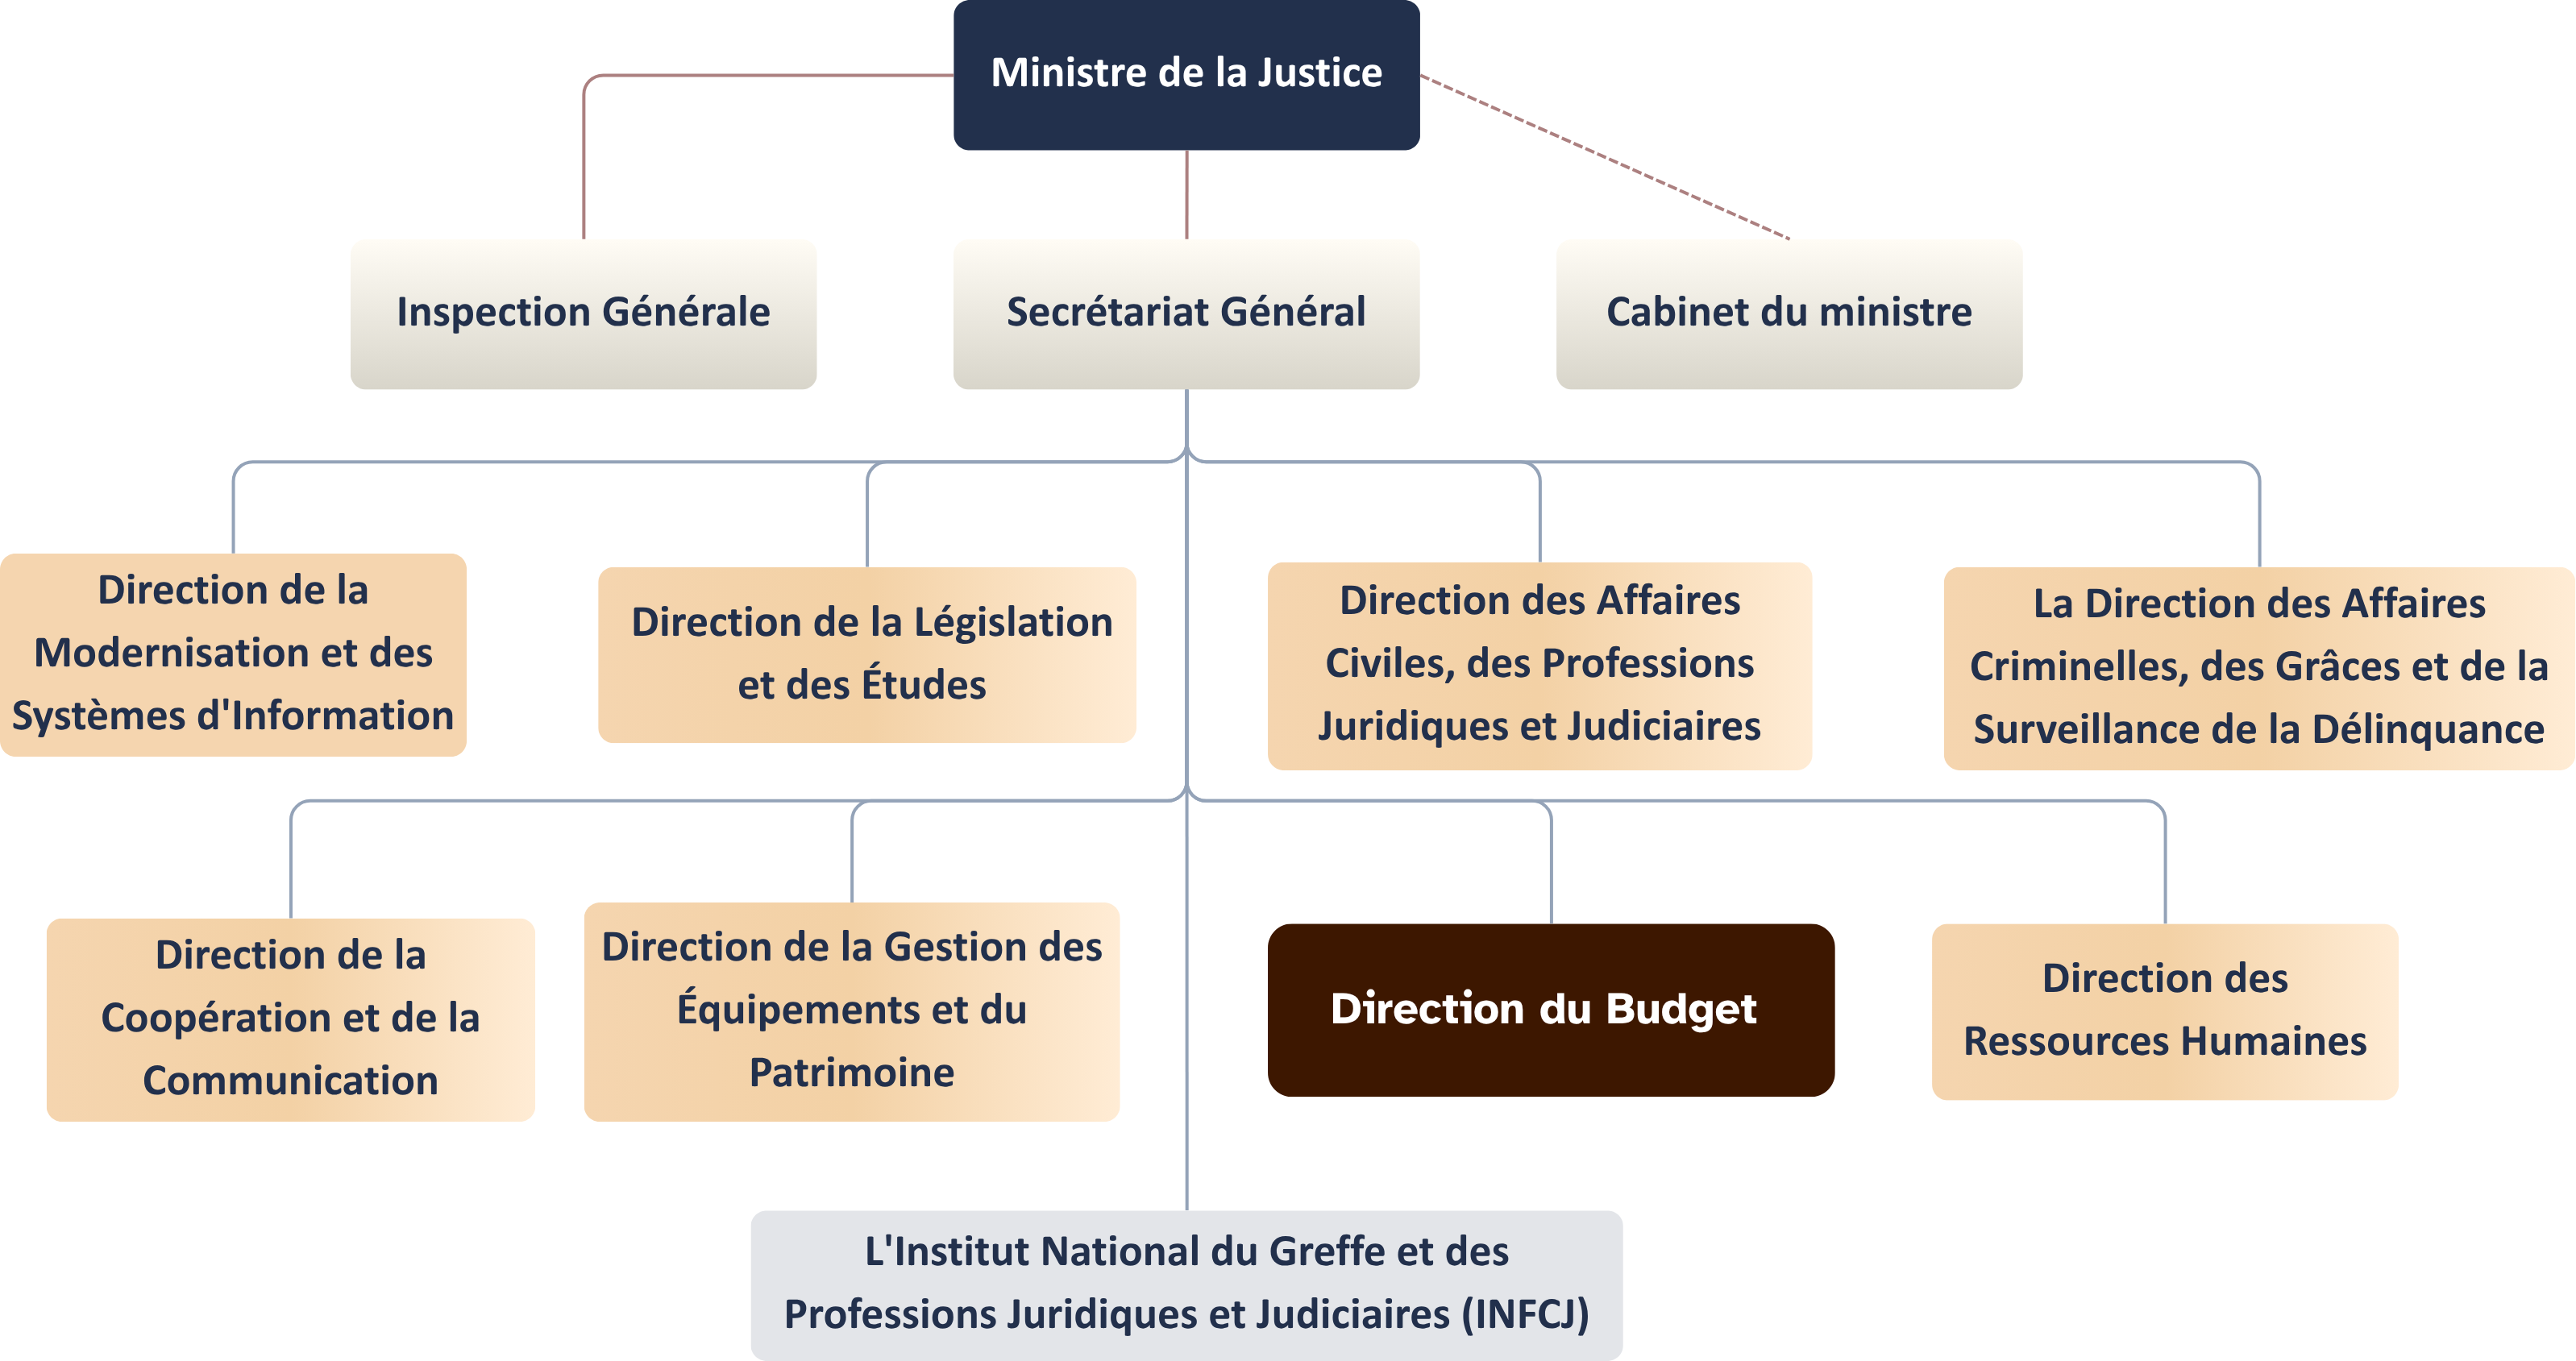
\includegraphics[width=\textwidth]{figures/organigrammeJustice.png}
\caption{Organigramme du minist\`ere de la Justice (source~: D\'ecret n\textsuperscript{o}~2.22.400).}
\label{fig:organigramme_ministere}
\end{figure}


Au sein du ministère, la Direction du Budget constitue l'interlocuteur principal avec le ministère de l'Économie et des Finances (MEF) et la Trésorerie Générale du Royaume (TGR). Son rôle est détaillé à la \hyperref[sec:direction-budget]{section~1.3}.
%----------------------------------------------------------------
\phantomsection
\subsubsection*{1.2.2 \quad Services d\'econcentr\'es}
\addcontentsline{toc}{subsubsection}{1.2.2 Services d\'econcentr\'es}
%----------------------------------------------------------------

Les services d\'econcentr\'es constituent la composante op\'erationnelle de l'institution. Ils comprennent notamment~:

\begin{itemize}
    \item La Cour de cassation (si\`ege \`a Rabat), juridiction supr\^eme de l'ordre judiciaire ordinaire
    \item Les Cours d'appel et les Cours administratives d'appel, r\'eparties dans les grandes villes du Royaume
    \item Les Tribunaux de premi\`ere instance (TPI) et les sections de justice de proximit\'e
    \item Les Tribunaux administratifs et les Tribunaux de commerce
    \item Les \'etablissements p\'enitentiaires g\'er\'es par la Direction G\'en\'erale de l'Administration P\'enitentiaire et de la R\'einsertion (DGAPR)
\end{itemize}

L'ensemble du r\'eseau judiciaire couvre les douze r\'egions du Royaume, avec des implantations dans la quasi-totalit\'e des provinces et pr\'efectures. Cette pr\'esence territoriale \'etendue explique en grande partie la complexit\'e logistique et budg\'etaire de l'institution~: des ordonnateurs secondaires d\'econcentr\'es re\c{c}oivent d\'el\'egation de cr\'edits et ex\'ecutent localement le budget, ce qui multiplie les flux budg\'etaires \`a suivre et \`a anticiper.

%================================================================
\phantomsection
\label{sec:direction-budget}
\subsection*{1.3 \quad La Direction du Budget}
\addcontentsline{toc}{subsection}{1.3 La Direction du Budget}
%================================================================

%----------------------------------------------------------------
\phantomsection
\subsubsection*{1.3.1 \quad Composition et positionnement}
\addcontentsline{toc}{subsubsection}{1.3.1 Composition et positionnement}
%----------------------------------------------------------------

Au sein de l'organigramme minist\'eriel, la Direction du Budget joue un r\^ole central dans la gestion des ressources financi\`eres de l'institution. Rattach\'ee hi\'erarchiquement au Secr\'etariat G\'en\'eral, elle constitue l'interface principale entre le minist\`ere de la Justice d'une part, et le MEF et la TGR d'autre part.

\paragraph{Composition~:}

Conform\'ement \`a l'article~30 du d\'ecret organisant les structures du minist\`ere (B.O.\ n\textsuperscript{o}~7161), la Direction du Budget comprend les entit\'es suivantes~:

\begin{itemize}
    \item \textbf{Division de la gestion du budget et de la comptabilit\'e} (\textit{qism tadbir al-miz\^aniyya wa-l-muh\^asaba})~: gestion des engagements de d\'epenses et des paiements, suivi des comptes affect\'es \`a des fins sp\'eciales, d\'el\'egations de cr\'edits aux ordonnateurs secondaires, et \'elaboration des situations annuelles d'ex\'ecution budg\'etaire.

    \item \textbf{Division des comptes des tribunaux} (\textit{qism his\^ab\^at al-mah\^akim})~: suivi et centralisation des comptes des tribunaux, gestion des comptables assign\'es aux caisses des tribunaux, et suivi des paiements \'electroniques.

    \item \textbf{Division du recouvrement} (\textit{qism al-tah\d{s}\^il})~: suivi du recouvrement des amendes et condamnations p\'ecuniaires, des frais et d\'epens judiciaires, et des paiements \'electroniques li\'es aux op\'erations de recouvrement.

    \item \textbf{Division de la pr\'evision et de la programmation financi\`ere} (\textit{qism al-tawaqqu\textquoteleft{} wa-l-barmaja al-m\^aliyya})~: \'elaboration des programmes budg\'etaires pluriannuels et du projet de budget annuel du minist\`ere, pr\'eparation du projet de performance et du rapport de nageât al-ad\^a\textquoteleft, conduite du dialogue de gestion avec les tribunaux, et pr\'evision, suivi et \'evaluation de l'ex\'ecution budg\'etaire.

    \item \textbf{Service des affaires techniques et logistiques} (\textit{masla\d{h}at al-shu\textquoteleft\^un al-tiqniyya wa-l-lujistikiyya})~: appui technique et logistique aux divisions de la direction.
\end{itemize}

C'est la \textbf{Division de la pr\'evision et de la programmation financi\`ere} qui constitue le terrain direct de notre recherche~: elle produit les pr\'evisions budg\'etaires annuelles et triennales et dispose de l'historique d'ex\'ecution n\'ecessaire \`a la mod\'elisation.

\begin{figure}[H]
\centering
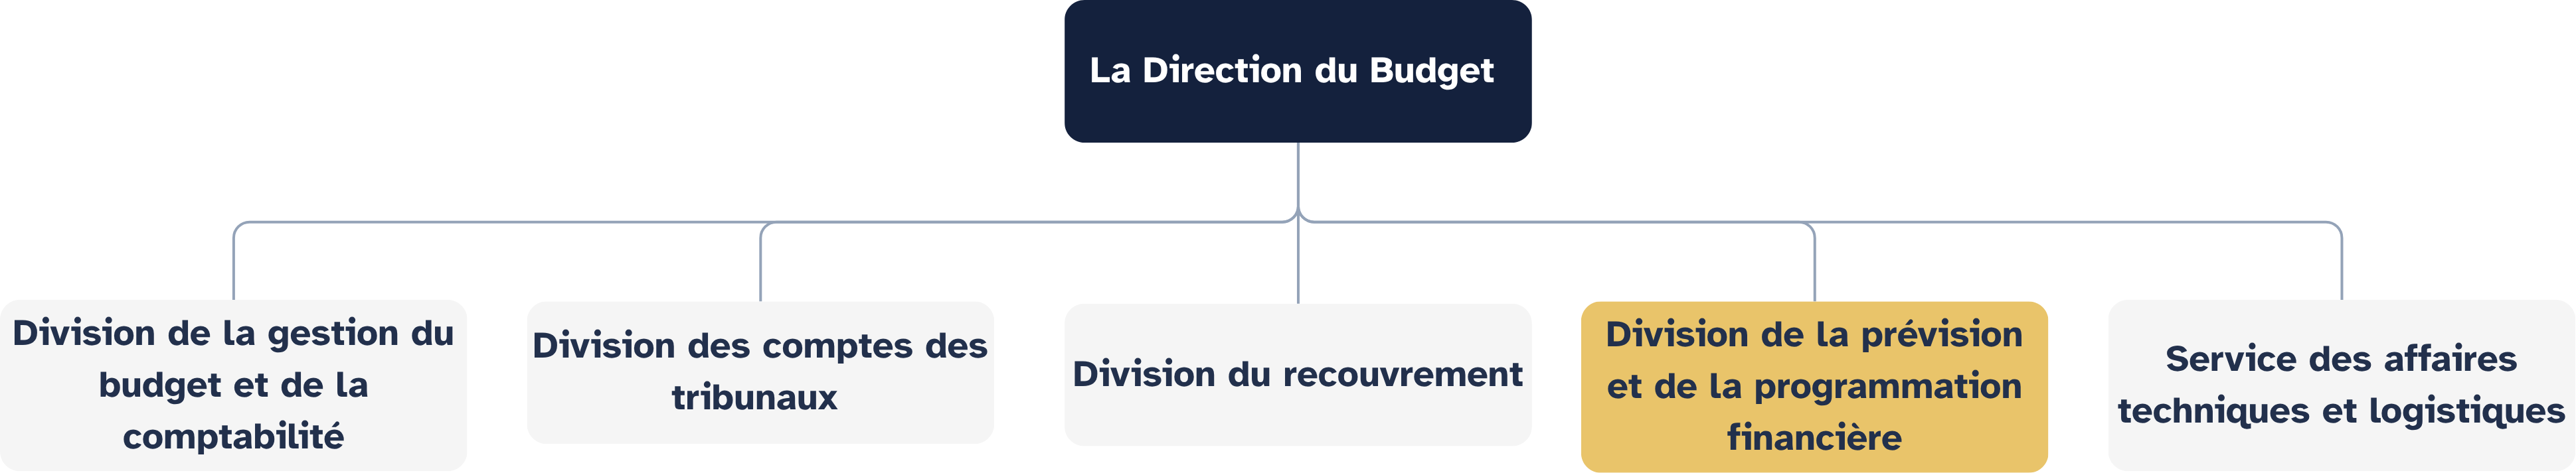
\includegraphics[width=0.95\textwidth]{figures/figure2.png}
\caption{Structure de la Direction du Budget du minist\`ere de la Justice.}
\label{fig:organigramme_db}
\end{figure}



%----------------------------------------------------------------
\phantomsection
\subsubsection*{1.3.2 \quad Fonctions et interfaces}
\addcontentsline{toc}{subsubsection}{1.3.2 Fonctions et interfaces}
%----------------------------------------------------------------

Les fonctions de la Direction du Budget couvrent l'ensemble du cycle de vie budg\'etaire~:

\begin{itemize}
    \item \textbf{La programmation budg\'etaire}~: coordination de l'\'elaboration des projets de performance annuels et triennaux (PBT-CDMT), consolidation des besoins remont\'es par les directions centrales et les services d\'econcentr\'es, et d\'efense des demandes de cr\'edits lors des conf\'erences budg\'etaires avec la Direction du Budget du MEF.

    \item \textbf{L'ex\'ecution budg\'etaire}~: gestion des cr\'edits d\'el\'egu\'es, suivi des engagements, coordination avec les ordonnateurs secondaires d\'econcentr\'es, et suivi du taux de consommation des cr\'edits en temps r\'eel via le syst\`eme GID de la TGR.

    \item \textbf{Le reporting et le contr\^ole de gestion}~: production des tableaux de bord budg\'etaires p\'eriodiques, renseignement des indicateurs de performance contractualis\'es avec le MEF, et alimentation des Rapports Annuels de Performance (RAP) transmis au Parlement conform\'ement \`a la LOF 130-13.

    \item \textbf{La gestion des archives d'ex\'ecution financi\`ere}~: extraction, compilation et archivage des \'etats d'ex\'ecution budg\'etaire mensuels produits par le syst\`eme GID, qui constituent la mati\`ere premi\`ere de notre analyse empirique (voir chapitre~3).

    \item \textbf{La gestion des restes \`a payer}~: suivi des engagements pluriannuels non encore sold\'es, coordination avec la TGR pour les ordonnancements diff\'er\'es, et pilotage de la tr\'esorerie budg\'etaire.
\end{itemize}

\paragraph{Interfaces externes~:}

Dans l'exercice de ses missions, la Direction du Budget interagit avec plusieurs acteurs ext\'erieurs au minist\`ere. La \textbf{Direction du Budget du MEF} fixe les enveloppes dans les lettres de cadrage et arbitre les demandes lors des conf\'erences budg\'etaires annuelles. La \textbf{TGR} assure l'ex\'ecution comptable et le contr\^ole des d\'epenses via le syst\`eme de Gestion Int\'egr\'ee de la D\'epense (GID), d\'eploy\'e depuis 2009 pour offrir une vision en temps r\'eel de l'\'etat de consommation des cr\'edits \citep{ElMoussali2023}. L'\textbf{Inspection G\'en\'erale des Finances (IGF)} proc\`ede \`a des audits p\'eriodiques de la gestion financi\`ere. La \textbf{Cour des Comptes} exerce le contr\^ole juridictionnel \textit{a posteriori} sur les comptes publics, et ses observations alimentent annuellement le dialogue de gestion entre le minist\`ere et le MEF.

C'est dans ce contexte que s'inscrit la probl\'ematique de ce m\'emoire. La Direction du Budget dispose d'un historique riche de donn\'ees d'ex\'ecution budg\'etaire, mais les m\'ethodes de pr\'evision conventionnelles restent insuffisamment adapt\'ees \`a la complexit\'e des dynamiques de d\'epense. Ceci soul\`eve la question centrale de notre recherche~:

\begin{center}
\textit{Dans quelle mesure les mod\'eles de Machine Learning peuvent-ils am\'eliorer
la pr\'evision du taux d'ex\'ecution budg\'etaire au sein du minist\'ere de la Justice,
et comment ces pr\'evisions peuvent-elles alimenter un syst\'eme d'aide \`a la d\'ecision
pour un pilotage proactif des cr\'edits en cours d'exercice~?}
\end{center}

Cette question ne postule pas que le Machine Learning \textit{surpasse} n\'ecessairement
les m\'ethodes statistiques classiques sur un crit\'ere de pr\'ecision brut~: elle
s'interroge sur la \textbf{valeur ajout\'ee op\'erationnelle} que ces outils peuvent
apporter \`a un gestionnaire budg\'etaire (d\'etection pr\'ecoce des lignes \`a risque,
generation de sc\'enarios, aide \`a la r\'eallocation des cr\'edits) l\`a o\'u une
simple moyenne historique ne fournit qu'une projection passive.

%----------------------------------------------------------------
\phantomsection
\subsubsection*{1.3.3 \quad La Division de Pr\'evision et de Programmation Financi\`ere}
\addcontentsline{toc}{subsubsection}{1.3.3 La Division de Prévision et de Programmation Financière}
%----------------------------------------------------------------

C'est au sein de cette direction, et plus pr\'ecis\'ement dans la \textbf{Division de Pr\'evision et de Programmation Financi\`ere} (\textit{qism al-tawaqqu\textquoteleft{} wa-l-barmaja al-m\^aliyya}), que s'est d\'eroul\'e notre stage. D\'efinie par l'article~34 du d\'ecret n\textsuperscript{o}~2.22.400\footnote{Bulletin Officiel n\textsuperscript{o}~7161 du 16~janvier~2023, page~485.}, cette division est investie des missions suivantes~:

\begin{enumerate}
    \item \textbf{\'Elaboration des programmes budg\'etaires pluriannuels et du projet de budget annexe annuel} du minist\`ere~: traduction des orientations strat\'egiques en enveloppes financi\`eres pluriannuelles (CDMT triennal) et construction du projet de budget pr\'epar\'e \`a l'occasion de chaque loi de finances.

    \item \textbf{Pr\'eparation du projet et du rapport de performance} (\textit{naja\textquoteleft{}at al-ad\^a\textquoteleft{}}) annex\'es au projet de loi de finances~: formalisation des objectifs strat\'egiques, d\'efinition des indicateurs et renseignement des cibles, conform\'ement aux exigences de la LOF~130-13.

    \item \textbf{Pr\'eparation et conduite du dialogue de gestion avec les tribunaux} (\textit{hiw\^ar al-tadbir ma\textquoteleft{}a al-mah\^akim})~: animation de la concertation annuelle avec les ordonnateurs secondaires d\'econcentr\'es pour la r\'epartition des cr\'edits et la n\'egociation des objectifs de performance.

    \item \textbf{\'Elaboration des programmes contractuels et suivi de leur ex\'ecution}~: mise en \oe{}uvre des engagements contractualis\'es avec le MEF, pilotage des programmes d'investissement pluriannuels et reporting p\'eriodique sur l'avancement physique et financier.

    \item \textbf{Pilotage financier des projets et coordination avec les partenaires institutionnels}~: gestion des partenariats, suivi des conventions de financement et articulation avec les bailleurs de fonds institutionnels.

    \item \textbf{Pr\'evision, suivi et \'evaluation de l'ex\'ecution budg\'etaire, et accompagnement des services d\'econcentr\'es} en mati\`ere financi\`ere et comptable~: c'est la mission \textit{cardinale} au regard de notre recherche. Elle implique la production de pr\'evisions de taux d'ex\'ecution \`a horizon mensuel et trimestriel, le suivi des \'ecarts entre cr\'edits ouverts et cr\'edits consomm\'es, et le conseil proactif aux ordonnateurs secondaires sur les risques de sous-ex\'ecution ou de d\'epassement.

    \item \textbf{Pr\'eparation du compte administratif et rapport sur l'ex\'ecution des d\'epenses budg\'etaires}~: cl\^oture annuelle du cycle budg\'etaire, consolidation des \'etats comptables finals et production du bilan d'ex\'ecution transmis au MEF et \`a la Cour des Comptes.
\end{enumerate}

C'est la mission~6 qui fonde directement l'utilit\'e op\'erationnelle de ce m\'emoire~: disposer de pr\'evisions d'ex\'ecution fiables et pr\'ecoces constitue, pour cette division, une exigence fonctionnelle permanente, que les m\'ethodes actuelles fond\'ees sur des extrapolations tendancielles ou des comparaisons \`a l'ann\'ee pr\'ec\'edente ne satisfont qu'imparfaitement.

%================================================================
\phantomsection
\subsection*{1.4 \quad Enjeux et objectifs du m\'emoire}
\addcontentsline{toc}{subsection}{1.4 Enjeux et objectifs du m\'emoire}
%================================================================

%----------------------------------------------------------------
\phantomsection
\subsubsection*{1.4.1 \quad Enjeux du projet}
\addcontentsline{toc}{subsubsection}{1.4.1 Enjeux du projet}
%----------------------------------------------------------------

Ce m\'emoire s'inscrit dans une d\'emarche qui d\'epasse le simple exercice acad\'emique~: il r\'epond \`a des enjeux concrets et imm\'ediats pour le minist\`ere de la Justice et, plus largement, pour la gouvernance financi\`ere publique au Maroc.

\begin{itemize}
    \item \textbf{Cr\'edibilit\'e budg\'etaire et redevabilit\'e parlementaire~:}
    La LOF~130-13 a institu\'e l'obligation pour chaque minist\`ere de produire un Rapport Annuel de Performance (RAP) pr\'esentant les r\'ealisations par rapport aux pr\'evisions. Des \'ecarts persistants entre pr\'evisions et ex\'ecution fragilisent la cr\'edibilit\'e de l'institution vis-\`a-vis du Parlement et de la Cour des Comptes~; ils signalent \'egalement un d\'eficit de pilotage interne. Le D\'ecret n\textsuperscript{o}~2-22-580 du 3~mars~2023 rend d\'esormais obligatoire, dans chaque d\'epartement minist\'eriel, un dispositif de contr\^ole de gestion destin\'e \`a \og{}v\'erifier, en permanence, l'atteinte des objectifs de performance au regard des ressources allou\'ees et \`a analyser les r\'esultats par rapport aux pr\'evisions\fg{} \citep{DecretCDG2023}. Am\'eliorer la qualit\'e pr\'edictive des pr\'evisions est donc un enjeu de gouvernance autant que de gestion.

    \item \textbf{Optimisation de l'allocation des ressources~:}
    Un minist\`ere dont les cr\'edits d'investissement sont syst\'ematiquement sous-consomm\'es en d\'ebut d'exercice et sur-sollicit\'es en fin d'ann\'ee subit un co\^ut d'opportunit\'e r\'eel~: des projets judiciaires (construction de tribunaux, \'equipement num\'erique) sont retard\'es, des restes \`a payer s'accumulent, et la qualit\'e du service public se d\'egrade. Une meilleure anticipation des flux permet une allocation plus fluide et plus efficiente des cr\'edits tout au long de l'ann\'ee budg\'etaire.

    \item \textbf{Positionnement dans la transformation digitale de l'administration~:}
    La Strat\'egie Nationale de D\'eveloppement des Donn\'ees Publiques et les orientations du Programme de R\'eforme de l'Administration placent la data et l'IA au c\oe{}ur de la modernisation de l'\'Etat. Le minist\`ere de la Justice, d\'ej\`a engag\'e dans la transformation num\'erique de ses services aux justiciables, peut \'etendre cette d\'emarche \`a son propre pilotage interne en exp\'erimentant des mod\`eles pr\'edictifs sur ses donn\'ees budg\'etaires.

    \item \textbf{Contribution \`a la recherche appliqu\'ee au contexte marocain~:}
    La litt\'erature sur l'application de l'IA \`a la pr\'evision des d\'epenses publiques est abondante au niveau international mais quasi inexistante pour le contexte marocain \`a l'\'echelle minist\'erielle. Ce travail contribue \`a combler cette lacune et peut servir de r\'ef\'erence m\'ethodologique pour d'autres d\'epartements minist\'eriels.
\end{itemize}

%----------------------------------------------------------------
\phantomsection
\subsubsection*{1.4.2 \quad Objectifs de la recherche}
\addcontentsline{toc}{subsubsection}{1.4.2 Objectifs de la recherche}
%----------------------------------------------------------------

Pour r\'epondre \`a ces enjeux, ce m\'emoire poursuit trois objectifs articul\'es~:

\begin{itemize}
    \item \textbf{Constituer et analyser une base de donn\'ees d'ex\'ecution budg\'etaire~:}
    Collecter, nettoyer et structurer les rapports trimestriels d'ex\'ecution budg\'etaire publi\'es par la Tr\'esorerie G\'en\'erale du Royaume (TGR) sur la p\'eriode 2020--2025 (24~observations), compl\'et\'es par les morasses annuelles extraites du portail \texttt{lof.finances.gov.ma}~; analyser les propri\'et\'es statistiques des s\'eries reconstitu\'ees (stationnarit\'e, saisonnalit\'e, effet COVID-19).

    \item \textbf{D\'evelopper et \'evaluer des mod\`eles de pr\'evision du taux d'ex\'ecution~:}
    Construire, calibrer et \'evaluer plusieurs mod\`eles, comprenant une r\'egression lin\'eaire r\'egularis\'ee (Lasso, puis Ridge apr\`es validation) et un algorithme de gradient boosting (XGBoost), ainsi que deux benchmarks na\"\i fs (d\'ecalage annuel et moyenne historique), selon un protocole de validation \textit{walk-forward} \`a fen\^etre expansive~; mesurer leurs performances relatives via des m\'etriques standardis\'ees (RMSE, MAE, MAPE)~; analyser ce que ces r\'esultats r\'ev\`elent sur la structure des d\'epenses du minist\`ere de la Justice.

    \item \textbf{Concevoir et impl\'ementer un syst\`eme d'aide \`a la d\'ecision op\'erationnel~:}
    D\'evelopper un tableau de bord interactif sous Power BI int\'egrant les pr\'evisions T4 ligne par ligne et un module de d\'etection d'anomalies fond\'e sur le score~$z$ du taux T2, illustrant comment les mod\`eles pr\'edictifs peuvent \^etre mobilis\'es au service du pilotage budg\'etaire courant et formuler des recommandations concr\`etes pour leur appropriation par les \'equipes de la Direction du Budget.
\end{itemize}

%----------------------------------------------------------------
\phantomsection
\subsubsection*{1.4.3 \quad Conclusion du chapitre}
\addcontentsline{toc}{subsubsection}{1.4.3 Conclusion du chapitre}
%----------------------------------------------------------------

Ce premier chapitre a permis de poser le cadre institutionnel et organisationnel dans lequel s'inscrit notre recherche. \`A travers la pr\'esentation du minist\`ere de la Justice (son histoire, ses missions, son organisation et la Direction du Budget qui en constitue le terrain direct), il est apparu que l'institution g\`ere un budget complexe, territorialement d\'econcentr\'e, soumis \`a des contraintes de performance croissantes depuis l'entr\'ee en vigueur de la LOF~130-13.

La Division de la pr\'evision et de la programmation financi\`ere produit des pr\'evisions budg\'etaires annuelles \`a partir de m\'ethodes qui restent, \`a ce jour, insuffisamment exploit\'ees par les outils quantitatifs disponibles. C'est pr\'ecis\'ement cette lacune que ce m\'emoire se propose de combler, en explorant comment les apports du Machine Learning peuvent \^etre int\'egr\'es dans le pilotage budg\'etaire~: non pas comme un substitut aux m\'ethodes existantes, mais comme un syst\`eme d'aide \`a la d\'ecision capable de travailler \`a la granularit\'e de la ligne budg\'etaire, de d\'etecter les anomalies en cours d'exercice, et de quantifier le risque de sous-ex\'ecution en temps r\'eel.

Le chapitre suivant approfondit le cadre budg\'etaire~: composition du budget, dispositif LOF, cycle d'ex\'ecution et d\'efis de la pr\'evision. Cette analyse permettra d'identifier avec pr\'ecision les s\'eries et les variables sur lesquelles repose notre mod\'elisation.

%================================================================\item \textbf{La transformation numérique et la modernisation du service judiciaire}~: dans le cadre du chantier de réforme inscrit dans la Charte Nationale pour la Réforme du Système Judiciaire, le ministère de la Justice œuvre à l'édification d'une administration judiciaire professionnelle, fondée sur la déconcentration administrative et financière et sur les piliers de la Justice numérique. La vision stratégique 2025--2030 place le justiciable au cœur de la transformation numérique, en visant à améliorer sa relation avec les juridictions, à garantir un accès équitable et égal au système juridique, et à mobiliser l'intelligence artificielle pour faciliter le travail de l'administration judiciaire \citep{MJNumerique2026}. Cette dynamique se concrétise par le déploiement de plusieurs plateformes numériques~: la plateforme de la \textit{Wissiqa el-Adliya} pour la dématérialisation des actes notariés liés au mariage, au divorce et aux successions~; la plateforme électronique de traitement des demandes de certificat de nationalité marocaine au bénéfice des Marocains résidant à l'étranger~; le portail de dépôt des demandes de grâce et de libération conditionnelle~; et la plateforme d'échange électronique de données interopérable avec les établissements bancaires et les sociétés d'assurance, en partenariat avec l'ACAPS et la Fédération Marocaine des Assurances.
